\documentclass[presentation]{subfiles}
\onlyinsubfile{
  \bibliography{references}
  \usepackage{tikz}
  \usetikzlibrary{positioning}
\renewcommand{\onlyinsubfile}[1]{}

}


\begin{document}


\begin{frame}\frametitle{Conceptual maps}
\centering
  \only<1>{\includegraphics[width=0.8\textwidth]{figures/tlitu/topo_world_scaled.jpg}\\\scriptsize{Topographical map by the NOAA}}
  \only<2>{\includegraphics[width=0.8\textwidth]{figures/tlitu/strava_heatmap_scaled.jpg}
    \\\scriptsize{Strava heatmap}}
\end{frame}








\begin{frame}[b]{Frustrations of reductive systems}
  \centering
  \includegraphics[width=0.5\textwidth]{figures/steps.png}

\end{frame}


\begin{frame}{How systems see us}
  

\begin{tikzpicture}[overlay]


\visible<+->{
  \node[xshift=2cm,yshift=-1cm] at (current page.south west)  (img00)                 {\includegraphics[width=0.4\textwidth]{figures/health_data/weight.png}};
}

\visible<+->{
  \node [above right=-3cm and -2cm of img00] (img01) {\includegraphics[width=0.4\textwidth]{figures/health_data/standhours.png}};
}

\visible<+->{
  \node [below right=-2cm and -4cm of img01] (img02)  {\includegraphics[width=0.4\textwidth]{figures/health_data/workout_time}};
  }


  \visible<+->{
  \node [above right=-2cm and -2cm of img02] (img03)  {\includegraphics[width=0.4\textwidth]{figures/health_data/heart_rate.png}};
  }

\end{tikzpicture}

\end{frame}







\begin{frame}{Living in {\bfseries Their} Utopia}
  
  \only<+>{\includegraphics[width=0.8\textwidth]{figures/tlitu/nyt_AI_FR.png}}
  \only<+>{\includegraphics[width=0.8\textwidth]{figures/tlitu/rapiscan.png}}
  % \only<+>{\includegraphics[width=0.8\textwidth]{figures/tlitu/nyt_AI_FR.png}}
  \only<+>{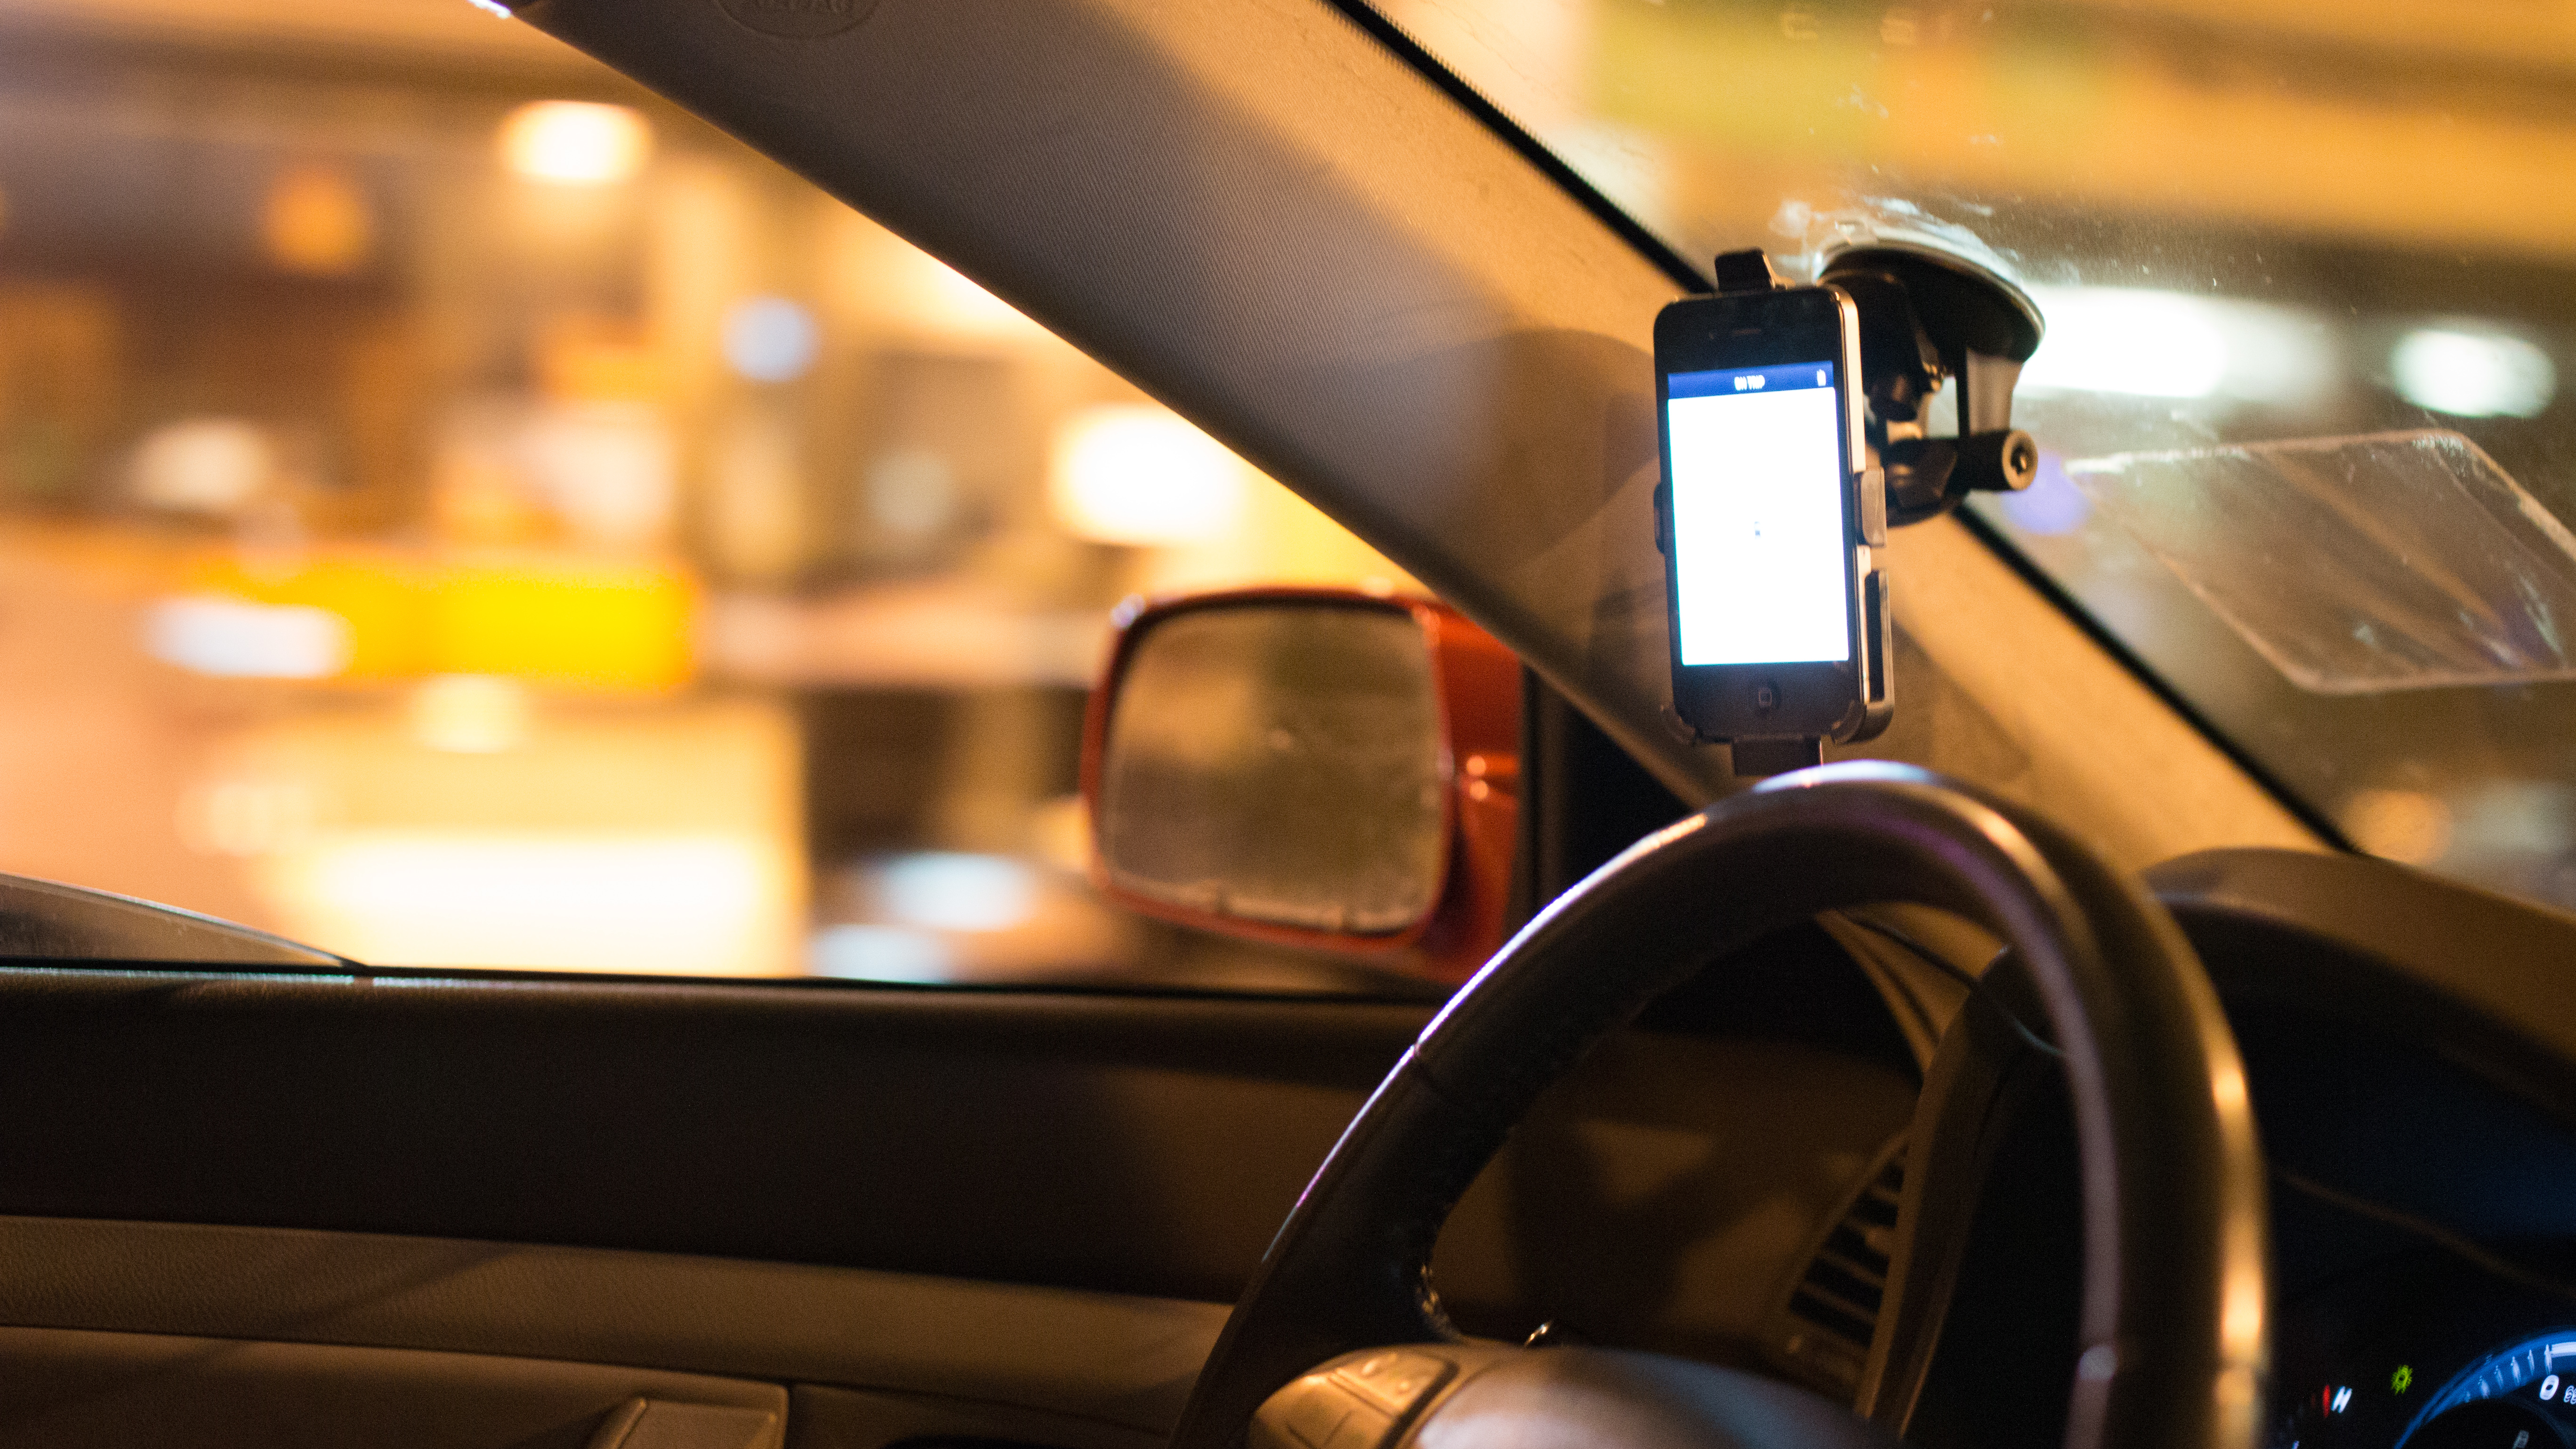
\includegraphics[width=0.8\textwidth]{../../common_figures/photo/gps-map.png}}
  % \only<+>{\includegraphics[width=0.8\textwidth]{}}
\end{frame}



\begin{frame}{takeaways}
  \begin{itemize}
    \item Disempower algorithms
    \item Find ways to help people escape the algorithm's absurdity
    \item Interrogate and continuously study the power dynamics unfolding
  \end{itemize}


\end{frame}



% \begin{frame}{towards ``thin description''}
  
%   \visible<2->{\renewcommand{\baselinestretch}{1.75}
%   \begin{tabular}{|p{0.9\textwidth}}
%   {\Large\itshape
%   [Thin description is] about how we all travel \dots through the thicket of time and space
%   }
%   \end{tabular}
% \renewcommand{\baselinestretch}{1}

%   \hfill-- \cite{jackson2013thin}}


%   \visible<3->{\renewcommand{\baselinestretch}{1.75}
%   \begin{tabular}{|p{0.9\textwidth}}
%   {\Large\itshape
%   [Thinness is] a methodological counterpoint to the hubris that animates so much tech development.
%   }
%   \end{tabular}
% \renewcommand{\baselinestretch}{1}

%   \hfill-- \cite{benjamin2019race}}


% \end{frame}



% \begin{frame}[plain]
%     \centering
% \visible<+->{We pass through so many \alert<1>{systems}, and \alert<1>{ecologies}, and \alert<1>{environments}, just like all the life of the forests scientists nearly destroyed}

% \visible<+->{It would be impossible, and \alert{hubris}, to try to capture and quantify all of that}

% \end{frame}

\end{document}



